\documentclass[10pt]{beamer}

\usetheme[progressbar=frametitle]{metropolis}
\usepackage{appendixnumberbeamer}
\usepackage{lipsum}
\usepackage{amsmath}
\usepackage{amssymb}
\usepackage{booktabs}
\usepackage[scale=2]{ccicons}
\usepackage{pgfplots}
\usepgfplotslibrary{dateplot}
\usepackage{dirtytalk}
\usepackage{xspace}
\newcommand{\themename}{\textbf{\textsc{metropolis}}\xspace}
\definecolor{mpigreen}{HTML}{007977}
\setbeamercolor{frametitle}{bg=mpigreen}
%https://www.overleaf.com/project/60692a72c2db80145723d37f
\title{Exploring Diseases Dataset \\for Chatbot Dialogue Management}

\author{Tai Ng. (Applied Scientist)}

\institute{VINBRAIN INTERNSHIP PROGRAM 2021 }
\titlegraphic{\hfill
\includegraphics[height=3cm]{logo.png}}

\begin{document}


\maketitle

\begin{frame}{Introduce Task Dialogue Systems}
\section{Characteristics}
A task-oriented dialogue system is developed to perform a clearly defined task. Usually, the task involves finding information within a database and returning it to the user, performing an action, or retrieving information from its users.
\end{frame}

\begin{frame}{Task Dialogue Systems}
\section{Technologies}
Usually, the user’s input is processed by a natural language understanding (NLU) unit, which extracts the slots and their values from the utterance and identifies corresponding the dialogue act. This information is passed to the dialogue state tracker (DST), which infers the current state of the dialogue. Finally the output of the dialogue manager is passed to a natural language generation (NLG) component.
\end{frame}

\begin{frame}{Introduce Task Dialogue Systems}
\section{Dialogue Management (DM)}

The DM could be connected to some external Knowledge Base (KB) or Data Base (DB), such that it can produce more meaningful answers.

The Dialogue Manager consists the following two components: 
\begin{itemize}
\item The Dialogue State Tracker 
\item Policy Learning
\end{itemize}
\end{frame}

\begin{frame}{Introduce Task Dialogue Systems}
\section{Approach Dialogue Management}
\begin{itemize}
\item Rule-based: Finite state machine 
\item Learning-based: Deep Q-Learning
\end{itemize}
\end{frame}

\begin{frame}{Introduce Task Dialogue Systems}
\section{Evaluation}
Two main aspects are evaluated, which have been shown to define the quality of the dialogue:
\begin{itemize}
    \item Task-success
    \item Dialogue efficiency
\end{itemize}

\end{frame}

\begin{frame}{Methods}
\section{Diseases Dataset}
A dataset to provide the students a source to create a healthcare related system.

\begin{figure}[H]
    \centering
    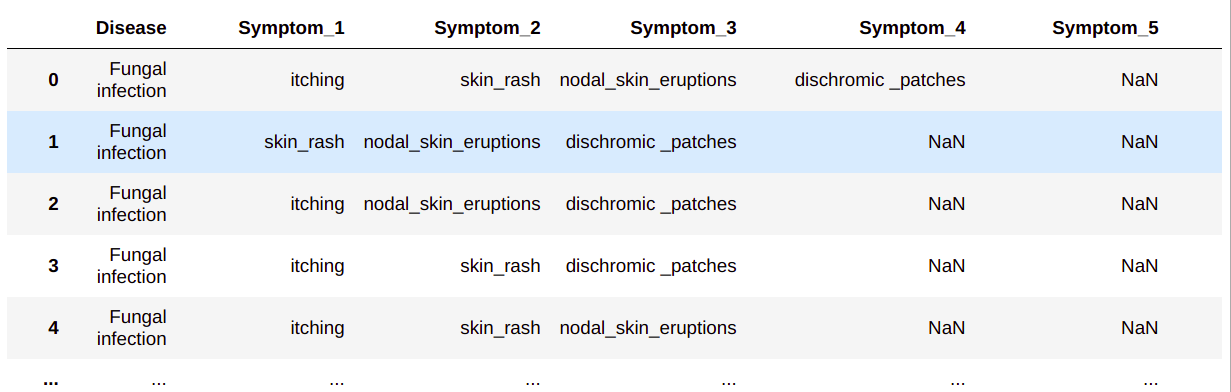
\includegraphics[width=10cm]{image/diseases_dataset.png}
    \caption{Diseases Dataset}
    \label{fig:di_ds}
\end{figure}

\end{frame}

\begin{frame}{Methods}
    \section{Insight}
    Investigate the correlation between each other diseases over the symptoms.
    \begin{itemize}
    \item Construct the chatbot script (usecase)
    \item Avoid waste of time to query KB/DB
    \item Define semantic frame for response task
    \end{itemize}
\end{frame}

\begin{frame}{Methods}
    \section{Database}
    \begin{figure}[H]
    \centering
    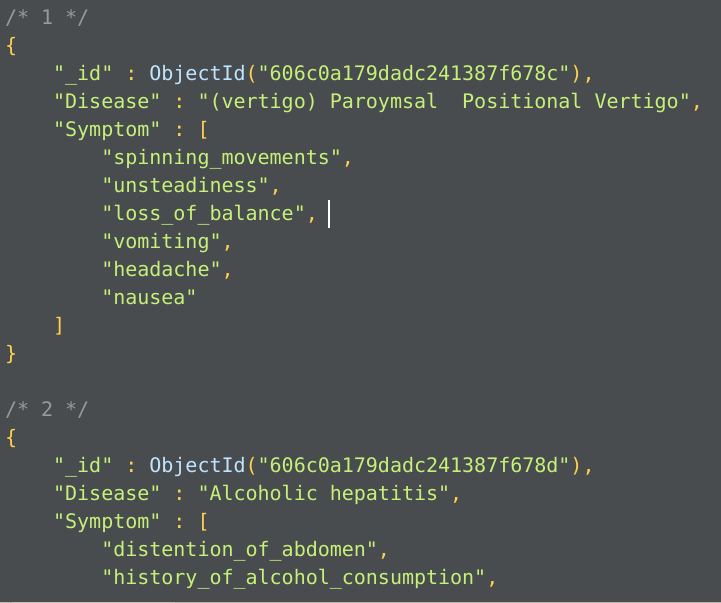
\includegraphics[width=5cm]{image/dbms.png}
    \caption{Disease database}
    \label{fig:di_dbms}
    \end{figure}
\end{frame}

\begin{frame}{Methods}
    \section{Dialogue tracking}
    \begin{figure}[H]
    \centering
    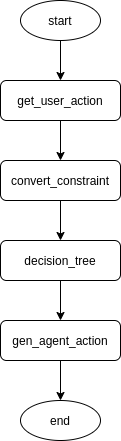
\includegraphics[width=2cm, angle=90]{image/flow_dm.png}
    \caption{Flow dialogue management}
    \label{fig:flow_dm}
    \end{figure}
\end{frame}

\begin{frame}{Methods}
    \section{Agent's action}
    \begin{enumerate}
        \item Inform \& Request: Randomly, amount of records greater than one.
        \item Match found: Only one record satisfy user's constraints.
        \item Done: End conversation if cannot found disease.
        
    \end{enumerate}
\end{frame}

\begin{frame}{Experiments}
    \section{API}
    \begin{figure}[H]
    \centering
    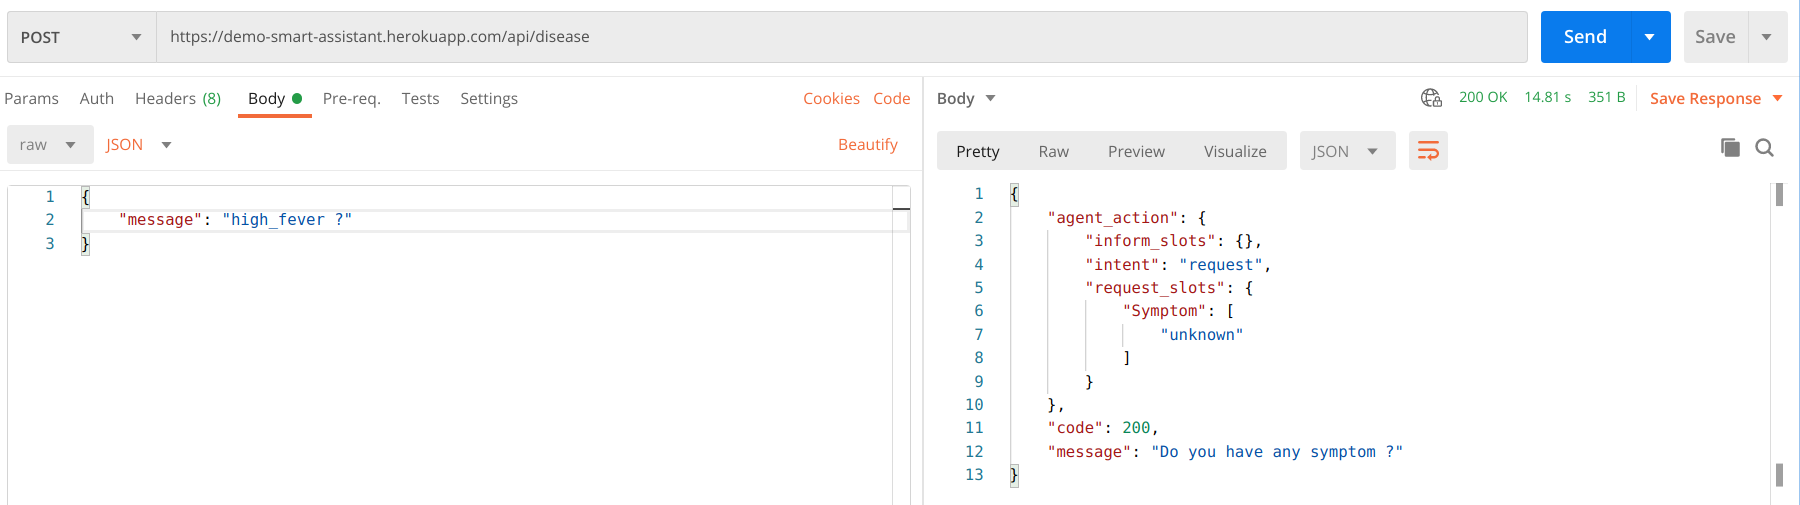
\includegraphics[width=10cm]{image/call_api.png}
    \caption{API}
    \label{fig:api}
    \end{figure}
\end{frame}

\begin{frame}{Experiments}
    \section{Demo}
    \begin{figure}[H]
    \centering
    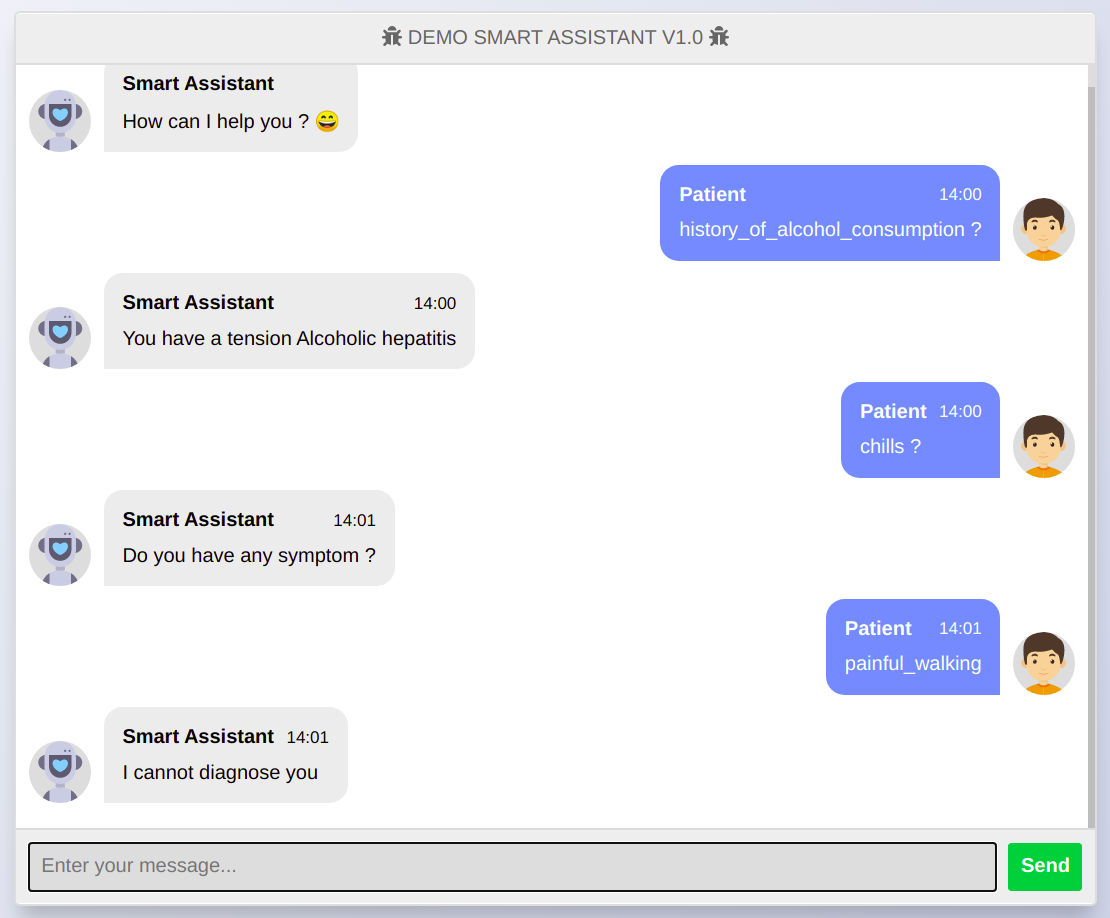
\includegraphics[width=7cm]{image/demo_smart_assistant.png}
    \caption{Demo conversation}
    \label{fig:demo}
    \end{figure}
\end{frame}

\begin{frame}{Conclusion}
    \begin{center}
        Q\&A
    \end{center}
\end{frame}

\end{document}
